%Hypothese 5: Die Einführung einer 4 Tage Woche führt zu einer Steigerung der 
Attraktivität des Arbeitgebers. 
%P&P

\chapter{Überprüfung der Hypothese 5}
\label{chap:hypothese5}


\section{Vorgehensweise}
Mit der Hypothese \gqq{Die Einführung einer 4-Tage-Woche führt zu einer 
Steigerung der Attraktivität des Arbeitgebers} wird - wie schon in \ref{tab:hyptothesen} beschrieben - der 
Fokus auf die Auswirkung der 4-Tage-Woche auf die Arbeitgebenden gelegt. 

\paragraph{Identifikation der relevanten Variablen}
In einem ersten Schritt werden die Variablen aus der durchgeführten Umfrage identifiziert, die für die 
Überprüfung der Hypothese relevant sind.

Als erstes ist dort die Frage \gqq{Könnte die Implementierung einer 4-Tage-Arbeitswoche die Attraktivität 
Ihres Unternehmens / Ihrer Organisation steigern?} zu nennen. Diese dient für die folgende Analyse als abhängige 
Variable, da sie die wahrgenommene Attraktivität des Arbeitgebenden in der untersuchten Stichprobe abbildet.

Zu den unabhängigen Variablen zählen in diesem Fall die Fragen, welche die Meinung der befragten 
Personen zur Attraktivität ihres Arbeitgebenden beeinflussen könnten. Diese sind:
% Demographische Faktoren
\begin{itemize}
  \item Alter
  \item Geschlecht
  % \item (Beschäftigungsverhältnis)
  \item Branche
  \item (Körperliche Beanspruchung)
  \item Die Position im Unternehmen (Führungskraft oder nicht)
\end{itemize}

\paragraph{Ausgewählte Analyseverfahren} Begonnen wird mit der allgemeinen Betrachtung der Meinung 
aller Befragten um das generelle Stimmungsbild der Stichprobe zu ermitteln. Anschließend werden die Auswirkungen
der einzelnen Variablen, welche zuvor genannt worden sind, auf die Attraktivität des Arbeitgebenden untersucht.

Für die allgemeine Betrachtung wird ein Histogramm der abhängigen Variable erstellt, um die Verteilung 
der Antworten zu visualisieren. Um einen weiteren tieferen Einblick in die Daten zu erhalten, werden 
ebenfalls der Modalwert (Modus), Median und Mittelwert der Antworten berechnet.

In der weiteren Betrachtung wird die Auswirkung einzelner unabhängigen Variablen auf die Meinung zur 
Attraktivität des Arbeitgebenden untersucht. Hierfür wurden erstmalig Kreuztabellen erstellt, um erste
Zusammenhänge zu erkennen. Anschließend werden darauf aufbauend abhängig von der Beschaffenheit des Merkmals
weitere Analyseverfahren angewendet.

\section{Analyse}

Die allgemeine Meinung der Befragten zur Attraktivität des Arbeitgebenden wird in dem folgenden Histogramm 
\ref{fig:attraktivitaet_verteilung} dargestellt. Die Verteilung der Antworten zeigt, dass die Mehrheit der
Befragten die Einführung einer 4-Tage-Woche durch den Arbeitgebenden als attraktiv empfinden.

Das Histogramm zeigt jedoch eine klare Schieflage nach links, was widerspiegelt, dass die Verteilung 
asymmetrisch und die meisten Antworten im Bereich der höheren Attraktivität (1 - Ja und 2 - Eher Ja) liegen. 
Dies spiegelt sich auch im Mittelwert wieder, welcher mit 1,86 ebenfalls im Bereich der höheren Attraktivität
zu finden ist. Der Modalwert (Modus) liegt bei 1 (Ja), was bedeutet, dass die meisten Befragten die Einführung einer 
4-Tage-Woche als attraktiv beziehungsweise einen Arbeitgebenden, der dies tut, als attraktiv empfinden. Der Median
liegt bei 2 (Eher Ja), was ebenfalls auf eine positive Meinung der Befragten zur Attraktivität des Arbeitgebenden
hinweist.


\begin{figure}[h]
    \centering
    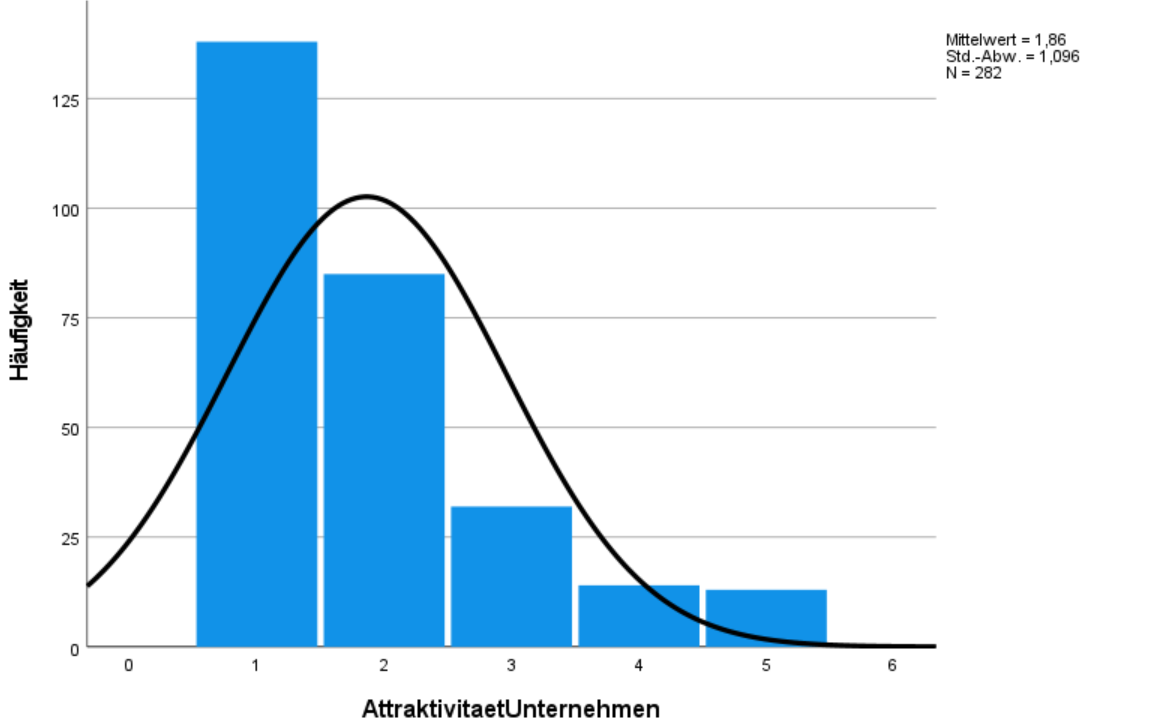
\includegraphics[width=0.7\textwidth]{04_Artefakte/01_Abbildungen/hypothese_5/attraktivitaet_histogram.png}
    \caption{Verteilung der Antworten zur Attraktivität des Arbeitgebenden}
    \label{fig:attraktivitaet_verteilung}
\end{figure}

Die weiteren explorativen Analysen zeigen, dass die Meinung zur Attraktivität des Arbeitgebenden besonders im 
Zusammenhand mit zwei Variablen zu stehen scheint: dem Geschlecht und ob die befragte Person eine Führungskraft ist oder nicht.
Die Forschenden hatten zu Beginn zwar auch einen Zusammenhang mit dem Alter der Befragten erwartet, jedoch konnte dies anhand
der Stichprobe nicht bestätigt werden da sich die Meinung zur Attraktivität des Arbeitgebenden nicht signifikant zwischen den 
Altersgruppen unterschied.
Darüber hinaus jedoch auch die Branche einen Einfluss auf die Meinung zur Attraktivität des Arbeitgebenden unter einer 4-Tage-Woche
zu haben, allerdings war die Stichprobe in diesem Fall zu klein, um belastbare Aussagen treffen zu können.

\subsection{Geschlecht}


\subsection{Führungskraft}


\section{Ergebnis}